%LTeX: language=de-DE
\chapter{Datenbank}
Für die Persistierung der Daten wird eine ''PostgreSQL\footnote{https://www.postgresql.org}'' Datenbank verwendet, die mithilfe von ''Docker\footnote{https://www.docker.com}'' in einem Container auf Port 5432 läuft. Die objektrelationale Abbildung der Objekte auf die Datenbank wird mit ''TypeORM\footnote{https://typeorm.io}'' durchgeführt.


\section{Main.ts}
Die Datei ''main.ts'' im Verzeichnis ''packages/database/src'' dient als Einstiegspunkt. Folgende Aufgaben werden hier ausgeführt:
\begin{itemize}
    \item Konfiguration, Erstellen und Export des Objektes ''AppDataSource''. Dieses Objekt wird später in der ''main.ts'' des Backends wieder importiert. ''AppDataSource'' ist dabei ein Objekt, das aus der Klasse ''DataSource'' gebaut wird welche aus dem ''TypeORM'' Modul stammt.
    \item Bauen der Repositories für jede Entität mit ''AppDataSource.getRepository()''. Die dafür nötigen Klassen der Entities werden aus dem ''entities'' Verzeichnis exportiert.
    \item Export der ''getEntityOrFail'' Methoden, welche in den ''Services'' im Backend verwendet werden.
\end{itemize}


\section{Entities}
Im Verzeichnis ''packages/database/src/entities'' liegt für jede Entity vom Datenmodell eine ''.ts'' Datei. In jeder dieser Dateien werden zuerst die nötigen Funktionen von ''TypeORM'' importiert. Danach folgt der Import der jeweiligen Entität aus dem ''Common'' Package. Weiters werden noch aus anderen Entitäten des ''entities'' Verzeichnisses jene Entities importiert, die in einer Beziehung zur aktuellen Entität stehen. Wie auch im Common Package und Backend Package wird auch hier viel mit ''Dekoratoren'' wie zum Beispiel ''@Entity'' gearbeitet, um dem darunterliegenden Code, Metadaten hinzuzufügen. Jedes Entity Klasse erbt von dem jeweiligen Import aus dem ''Common'' Package und ist mit ''@Entity'' ausgestattet, um eine Tabelle in der Datenbank zu repräsentieren. Für die Spalten werden ''@PrimaryColumn'' (PK) und @Column verwendet und mit ''ColumnOptions'' zusätzlich konfiguriert. So kann beispielsweise gesetzt werden, ob eine Spalte leer bleiben darf, einen Defaultvalue hat oder welche Zustande die Property haben kann wie zum Beispiel: ''enum: [manager, engineer, customer]''. Die Properties werden mit ''override name: datentyp'' angegeben. Mit ''@OneToMany'' bzw. ''@ManyToOne'' können 1:n bzw. n:1 Beziehungen zwischen den Tabellen definiert werden. Die nachfolgende Abbildung [siehe Abb. \ref{fig: dbentity} auf S.~\pageref{fig: dbentity}] zeigt, als Beispiel, die Implementierung der Entity ''Member''.

\begin{figure}[h]
    \centering
    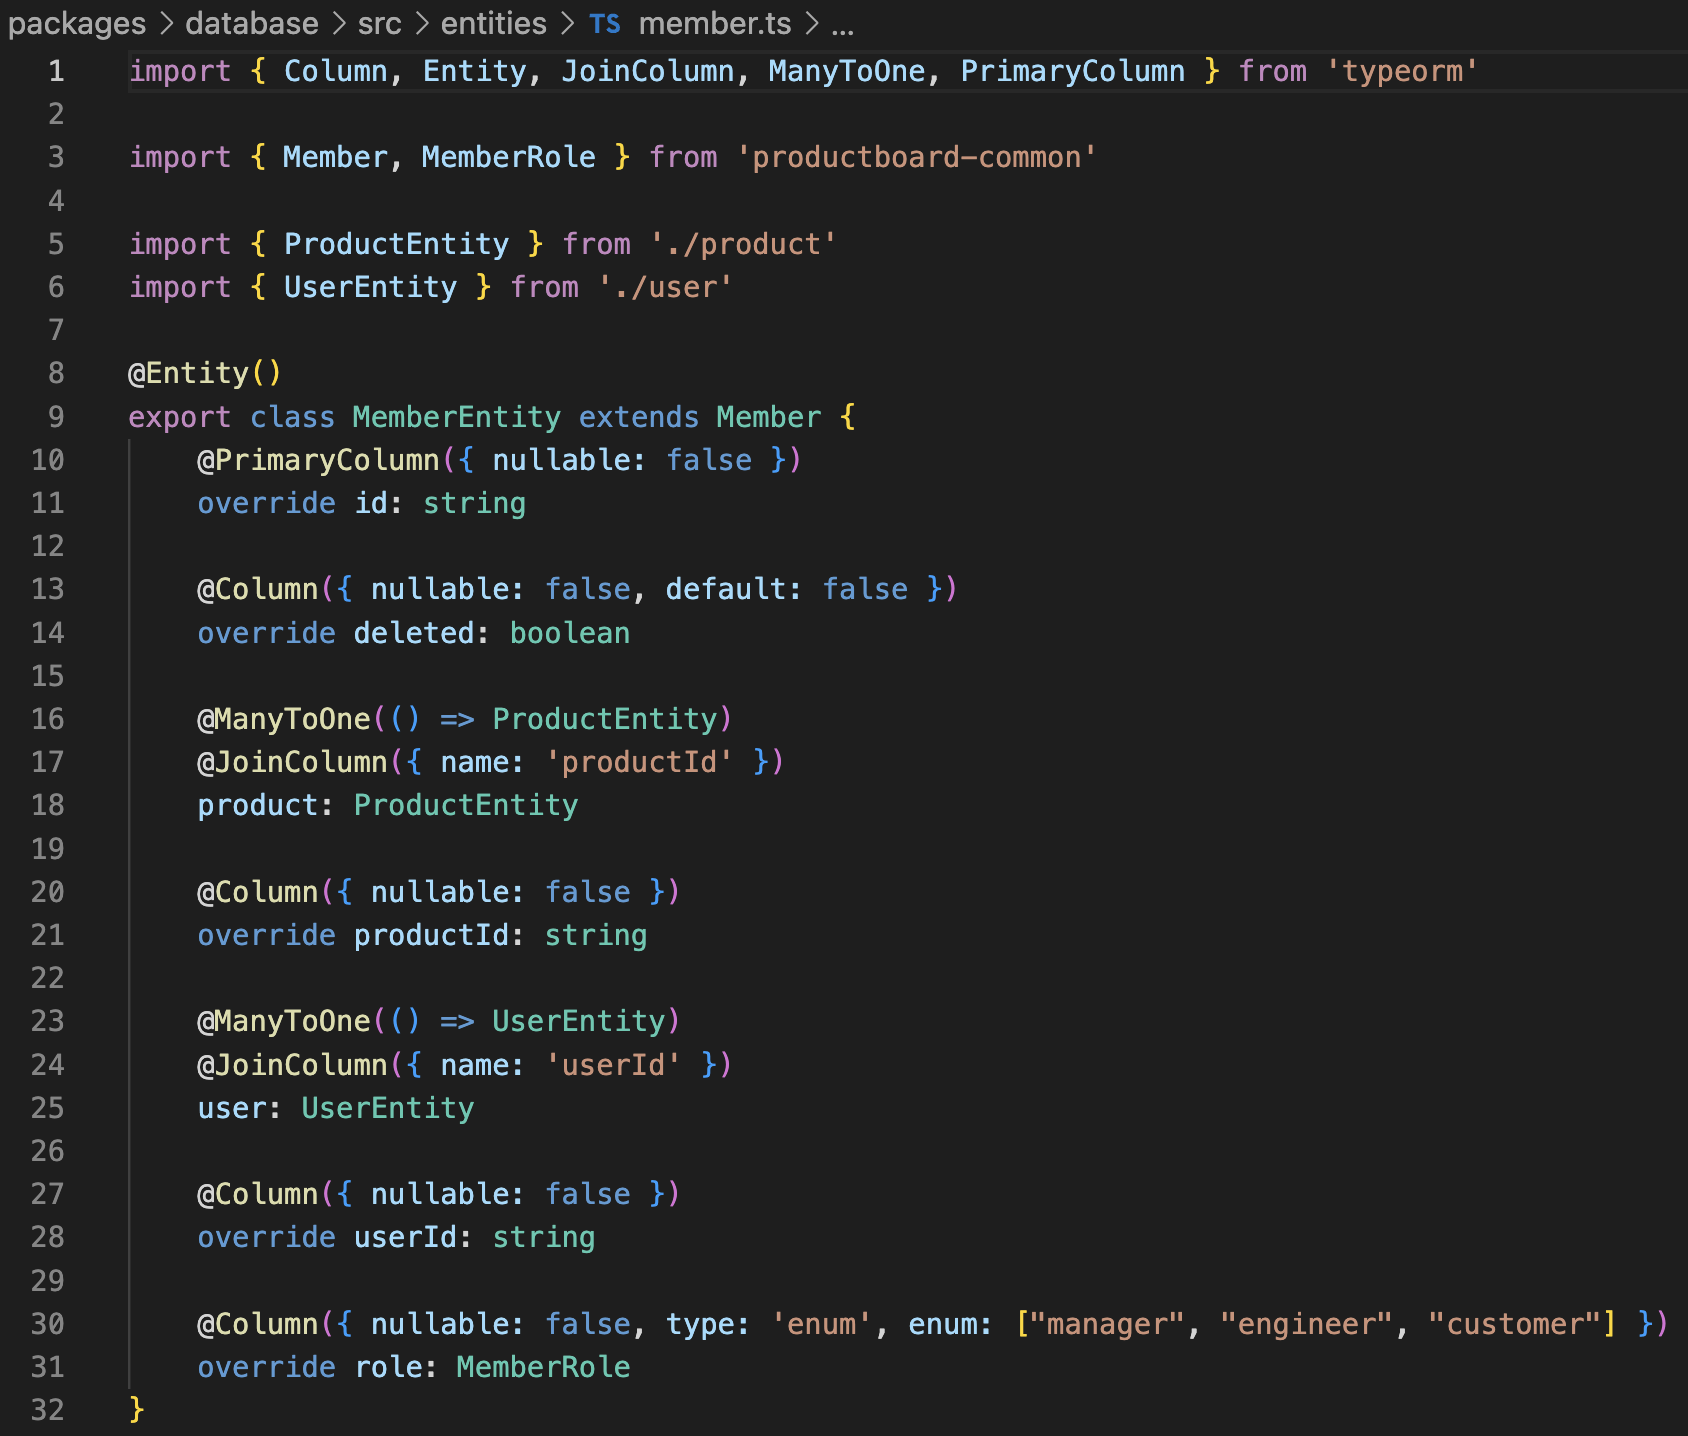
\includegraphics[width=1\textwidth]{dbentity.png}
    \caption{Member Entity.tsx}
    \label{fig: dbentity}
\end{figure}



